%
% File coling2020.tex
%
% Contact: feiliu@cs.ucf.edu & liang.huang.sh@gmail.com
%% Based on the style files for COLING-2018, which were, in turn,
%% Based on the style files for COLING-2016, which were, in turn,
%% Based on the style files for COLING-2014, which were, in turn,
%% Based on the style files for ACL-2014, which were, in turn,
%% Based on the style files for ACL-2013, which were, in turn,
%% Based on the style files for ACL-2012, which were, in turn,
%% based on the style files for ACL-2011, which were, in turn, 
%% based on the style files for ACL-2010, which were, in turn, 
%% based on the style files for ACL-IJCNLP-2009, which were, in turn,
%% based on the style files for EACL-2009 and IJCNLP-2008...

%% Based on the style files for EACL 2006 by 
%%e.agirre@ehu.es or Sergi.Balari@uab.es
%% and that of ACL 08 by Joakim Nivre and Noah Smith

\documentclass[11pt]{article}
\usepackage{coling2020}
\usepackage{times}
\usepackage{amsmath,amsfonts,amssymb}
\usepackage{url}
\usepackage{latexsym}
\usepackage{hyperref}
\usepackage[noabbrev,capitalize]{cleveref}
\usepackage{graphicx}
\usepackage{natbib}

%\setlength\titlebox{5cm}
\colingfinalcopy % Uncomment this line for the final submission

% You can expand the titlebox if you need extra space
% to show all the authors. Please do not make the titlebox
% smaller than 5cm (the original size); we will check this
% in the camera-ready version and ask you to change it back.


\title{Composing Byte-Pair Encodings for Morphological Sequence Classification}

\author{Adam Ek,\\
	Centre for Linguistic Theory and Studies in Probability,\\
	Department of Philosophy, Linguistics and Theory of Science,\\
	University of Gothenburg,\\
	\texttt{adam.ek@gu.se}}

\date{}

\begin{document}
	\maketitle
	
	\section{Introduction}
	\label{intro}
	
	\textbf{Things added to model:}
	\begin{itemize}
		\item Layer attention
		\item Adaptive learning rate
		\item Label smoothing
		\item Fine-tuning
		\item Dropouts
		\item Trained character representations (?)
	\end{itemize}
	
	\textbf{Things to add:}
	\begin{itemize}
		\item (results) More detailed accuracy for len(BPE)$>2$
		\item (results) With fine-tuning/without fine-tuning
		\item (data) Data statistics: number of MSD-tags 
		\item (data) Pick other datasets, try to match dataset sizes better (100k~150k train examples, turkish very small atm)
	\end{itemize}
    
    In this project we explore the transformer model applied to sequence classification. In sequence classification a dataset is split into words (or tokens) and each word is assigned a label. 
    Neural model can predict the label of a word by assigning it a representation and passing it through the network. However, the transformer model use byte-pair encoding (BPE) \cite{sennrich2015neural}, or some variation of it \citep{devlin2018bert}, to tokenize text. 
    BPE tokens are sub-strings that occur significantly often in the corpus, and does not correspond directly to words. For example, the word "scientifically" may be composed of the the BPE tokens: ["scient", "ifical", "ly"].
    %
    In sequence classification, we need to assign a label to the word "scientifically". But the word is now composed of three BPE embeddings, so to predict a label for the word we need to compose all of the BPE embeddings into one representation.
    
    In this project is to explore six different methods of creating word representations from multiple BPE embeddings.
	
%%%
    %Typically, the transformer model use some variation of byte-pair endings (BPE)  to split sentences into tokens. For non-bpe tokenization schemas typically words are selected based on white-space. This is convenient in sequence classification or parsing where for each word some label is assigned. 
    %In the BPE schema on the other hand a word (which has a label attached to it in some dataset) may be split into two or more BPE-tokens. 
    %The BPE vocabulary is usually selected such that significantly common sub-strings are saved. To create words using a BPE vocabulary, sub-strings are combined with each other.
    
    %In this project we explore how to compose embeddings of BPE tokens into word representations. More specifically, in cases when a word is associated with several BPE embeddings (for example: the word "scientifically" may be composed of the the BPE tokens: ["scient", "ifical", "ly"]) how do we combine the BPE embeddings to create a word representation ("scientifically") which we assign a label to.
    
    \paragraph{Task:} We explore combination of BPE embeddings with the task of Morphological-Tagging-in-Context \citep{mccarthy2019sigmorphon}. 
    The task is simply to predict the morphological features (such as case, number person, ...) of each word (as defined in the dataset) given the sentence which the word occur in.
    
    \paragraph{Data:} For the task we will use the Universal Dependencies dataset \citep{nivre2018} annotated with the UniMorph schema \citep{mccarthy2018marrying}. We look at 6 different languages: Arabic, Basque, Finnish, Czech, Spanish and Turkish. The language typology, ratio of BPE-tokens per word and training/development and test data can be found in \cref{tab:data}.
    
    	\begin{table}[h]
		\centering
		\begin{tabular}{l|lrrrr}
			Language & Typology & BPE-word ratio & Train & Validation & Test \\
			\hline
			Arabic-PADT  & Fusional & 1.39 & 225494 & 28089 & 28801  \\
			Basque-BDT  & Agglutinative & 1.79 & 97336 & 12206 & 11901 \\
			Czech-CAC   & Fusional & 1.77 & 395043 & 50087 & 49253 \\
			%English-EWT & Fusional & 1.33 & 204857 & 24470 & 25527 \\
			Finnish-TDT & Agglutinative & 1.98 & 161791 & 19876 & 20541 \\
			Spanish-AnCora & Fusional & 1.34 & 439925 & 55196 & 54449 \\
			Turkish-IMST & Agglutinative & 1.73 & 46417 & 5708 & 5734 \\
		\end{tabular}
		\caption{\label{tab:data} Treebank statistics.}
	\end{table}
    
    \paragraph{Base model}
    
	For the task we will use the XLMR \citep{conneau2019unsupervised} model\footnote{We use the fairseq implementation: \url{https://github.com/pytorch/fairseq/tree/master/examples/xlmr}}. XLMR is a masked language model based on the transformer (specifically, RoBERTa \citep{liu2019roberta}) trained on data from 100 different languages, using a shared vocabulary. In this experiment we use \textsc{XLMR}$_{LARGE}$, the model have 12 encoder layers, 16 attention heads and use 1024 dimensions for its hidden size.
	
	\section{Method}
	\label{method}
	
	In this section we present different methods of composing BPE embeddings into word representations and the structure of our neural network. We align BPE tokens to words by a simple string matching algorithm. 
	
	\subsection{Byte-pair combination methods}
	
	\paragraph{Sum:} For the sum method, we simply take the sum for each dimension of all BPE embeddings. Thus, for dimension $i$ we add all the values in all BPE embeddings $x_i^0 + ,..., + x_i^n$:
	
	\begin{equation}
	    x'_{i} = \sum_{j=1}^{n} x_i^j
	\end{equation}
	
		%\begin{equation}
		%	f(x) = \sum_{1}^{N} \sum_{1}^{d} x_d^0 + ... + x_d^n
		%\end{equation}
		
		%\begin{equation}
		%f(x) = \Big[(\sum_{1}^{n} x_0^0 + ... + x_0^n), ..., (\sum_{1}^{n} x_d^0 + ... %+ x_d^n)\Big]
		%\end{equation}
	
	\paragraph{Mean:} In the mean method we calculate the sum and divide by the number of BPE embeddings in the word. Thus, for dimension $i$ we calculate $\frac{x_i^0 + ,..., + x_i^n}{n}$: 
	
    	\begin{equation}
    	    x'_{i} = \frac{1}{n}\sum_{j=1}^{n} x_i^j
    	\end{equation}
		%\begin{equation}
		%	f(x) = \frac{1}{n}\Big[(\sum_{1}^{n} x_0^0 + ... + x_0^n), ..., %(\sum_{1}^{n} x_d^0 + ... + x_d^n)\Big]
		%\end{equation}
	
	\paragraph{Max:} In the max method we take the most activated value of dimension $i$ over all BPE embeddings $x^0...x^n$ in the word. 
	
		\begin{equation}
			x'_i = {argmax(x_i^0,...x_i^n)}
		\end{equation}
	
	\paragraph{RNN:} In this method we employ a bidirectional RNN to learn how to compose the BPE embeddings. For each multi-BPE token, we pass the sequence of BPE embeddings through an RNN and use the final output as the word representation.
	
	\paragraph{Att1:} In the first attention method we use self-attention \citep{vaswani2017attention} with one linear transformation. Like in the transformer we use three copies of the BPE sequence as inputs and transform one of them using a linear layer.
	We then calculate pairwise scores and apply softmax. We then use the softmax to create a weighted sum for the word representation.
	
	\begin{equation}
	    x = softmax(\frac{q (kW_k)^\intercal}{\sqrt{d}}) \cdot V
	\end{equation}
	
	\paragraph{Att3:} Like in the first attention method we use self-attentions. However, in the second attention approach we use three linear transformations, one for each copy of the input. 
	
	\begin{equation}
	    x = softmax(\frac{qW_q kW_k ^\intercal}{\sqrt{d}}) \cdot vW_v
	\end{equation}
	
	\subsection{Model}
	The model we employ use XLMR as a feature extractor, i.e. we only extract BPE embeddings from the model and do not fine-tune it. 
	%
	An outline of the model is presented in \cref{fig:model}, in the outline $f$ represent the different methods we use to combine BPE embeddings.
	
	\begin{figure}[h!]
		\centering
		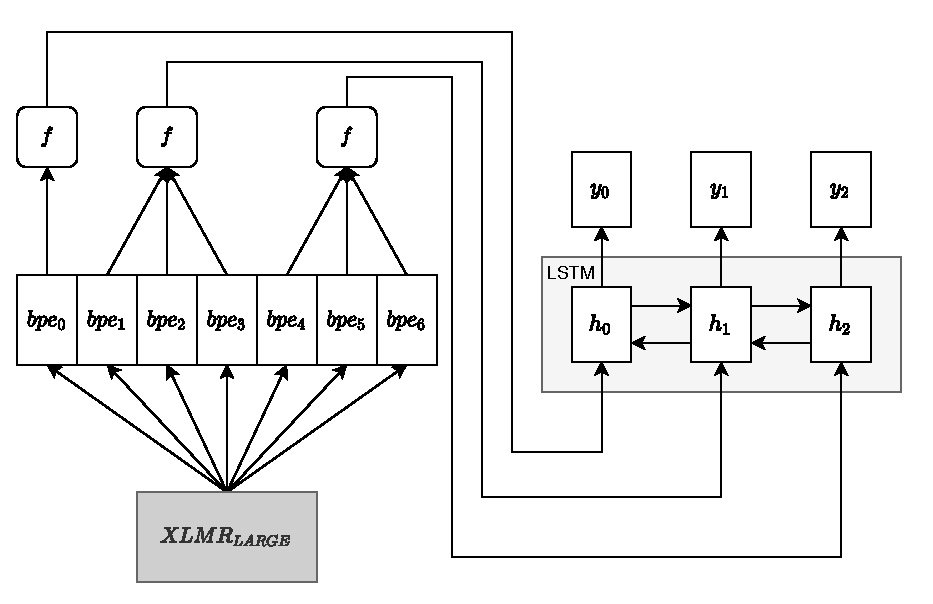
\includegraphics[scale=0.2]{model_outline-5.pdf}
		\caption{\label{fig:model} Procedure outline}
	\end{figure}
	
	The model we use to predict morphological features is simple. For each sentence we extract $n$ BPE embeddings from $XLMR_{LARGE}$ then align them to words. 
	We then run all words who consist of more than one BPE embedding through a function $f$ which combine the BPE embeddings. This produce one embedding per word which we pass to a bidirectional LSTM to extract contextual features. 
	We pass the LSTM outputs to a linear transformation layer that compute scores for each class in the output. We then apply softmax and compute the loss.

	
	\section{Results}
	\label{results}
	
	We present the results of our experiments in \cref{tab:results}. In general, our simple model using XLMR as a feature extractor yield good performance compared to the baseline. One exception is Basque, where the baseline is 0.1\% better than our model. 
	%
	We see the best improvement for Czech, where our model score above the baseline by 16.8\%. For the other languages, our best model increase the performance compared to the baseline by about 4\%.  
	
	In general the results indicate that combining BPE embeddings into word representations using a RNN works well for all languages. It achieves the best score for tokens overall for all six languages. 
	Looking at the accuracy of word representations containing two or more BPE embeddings, RNN also appear to work best. One exception is for Spanish-AnCora where Att3 performed marginally better (0.1\%) than the RNN method.
	
		\begin{table}[h]
		\small
		\centering
		\begin{tabular}{l|c|cccccc||cccccc}
			& &  \multicolumn{6}{c}{All Tokens Accuracy} & \multicolumn{6}{c}{BPE$>=2$ Accuracy} \\
			Treebank & Ratio & Sum & Mean & RNN & Att1 & Att3 & max & Sum & Mean & RNN & Att1 & Att3 & max \\
			\hline
			Finnish-TDT & .751 & .818 & .820 & \textbf{.833} & .821 & .822 & .817 & .738 & .739 & \textbf{.773} & .741 & .747 & 722 \\ 
			Basque-BDT & .676 & .652 & .659 & \textbf{.675} & 652 & .666 & .656 & .473 & .482 & \textbf{.525} & .474 & .499 & .478 \\
			Turkish-IMST & .620 & .623 & .626 & \textbf{.646} & .623 & .624 & .610 & .396 & .396 & \textbf{.449} & .396 & .410 & .368\\
			Spanish-AnCora & .842 & \textbf{.881} & .811 & \textbf{.881} & \textbf{.881} & .880 & .880 & .829 & .831 & .835 & .831 & \textbf{.836} & .828\\
			Arabic-PADT & .770 & .822 & .827&\textbf{.829}&.824&.825&.825&.709&.715&\textbf{.730}&.716&.718&.707\\
			Czech-CAC & .771 &.933 & .935 & \textbf{.939} & .933 & .935 &.914& .890 & .891 & \textbf{.905} & .890 & .893&.851\\
			
		\end{tabular}
		\caption{\label{tab:results} Accuracy for morphological tagging. Evaluated on all tokens and on all tokens that are composed of 2 or more BPE tokens.}
	\end{table}



	
	
	\section{Discussion}
        We can observe an interesting trend for the treebank samples. For the languages with agglutinative morphology\footnote{1-to-1 correspondence between morphemes and grammatical/syntactic features.} the average increase using RNN compared to Mean is 4.3\%. For the fusional\footnote{1-to-many correspondence between morphemes and grammatical/syntactic features.} languages, the difference between RNN and Mean is only 1.1\%. 
        
        Interestingly, this observation seem task-dependant rather than BPE dependant. We can see in \cref{tab:data} that Czech is a fusional language, but with a BPE-to-word ratio ($1.77$) comparable to the agglutinative languages. But, Czech also exhibit the pattern of benefiting less from RNN than from Mean, indicating that fusional languages\footnote{In our language/treebank sample.} regardless of BPE-to-word ratio is less affected by the composition method than agglutinative languages. 
        
        %In general, the agglutinative languages have a higher BPE-to-word ratio, with one exception, Czech. Czech have a BPE-to-word ratio of $1.77$, but still exhibit a lower difference between the RNN and mean method. Thus, from this small sample of treebanks it appears as if the method of combining BPE embeddings is more important for agglutinative languages than for fusional languages. 
        
	
	%\section*{Acknowledgments}
	
	
	% include your own bib file like this:
	\bibliographystyle{plain}
	\bibliography{coling2020}
	
\end{document}
